\state{Beta functions in Yukawa theory~(P\&S 12.1)}{
	In the pseudoscalar Yukawa theory studied in Problem~10.2, with masses set to zero,
	\eqn{lagr1}{
		\cL = \frac{1}{2} (\ptsm \phi)^2 - \frac{\lam}{4!} \phi^4 + \psib (i \ptsl) \psi - i g \psib \gamt \psi \phi,
	}
	compute the Callan-Symanzik $\bet$ functions for $\lam$ and $g$:
	\al{
		&\betl(\lam, g), &
		&\betg(\lam, g),
	}
	to leading order in coupling constants, assuming that $\lam$ and $g^2$ are of the same order.  Sketch the coupling constant flows in the $\lam$-$g$ plane.
}

\sol{
	The $\bet$ function of a generic dimensionless coupling constant $g$, associated with an $n$-point vertex, is given by P\&S~(12.53),
	\eqn{beta}{
		\bet(g) = M \pdv{M}( -\delg + \frac{1}{2} g \sumi \delZi),
	}
	where the sum is over the external legs.  This expression for $\bet$ implies P\&S~(12.54),
	\eqn{beta2}{
		\bet(g) = -2 B - g \sumi \Ai,
	}
	where~\cite[pp.~414--415]{Peskin}
	\aln{ \label{AB}
		\delZ &= A \ln(\frac{\Lam^2}{M^2}) + \finite, &
		\delg &= -B \ln(\frac{\Lam^2}{M^2}) + \finite;
	}
	$\Lam$ being a momentum cutoff and $M$ being the renormalization scale at which we define the theory~\cite[p.~408]{Peskin}.  Both Eq.~\refeq{beta} and Eq.~\refeq{beta2} hold for the $\bet$ function of Yukawa theory~\cite[p.~415]{Peskin}.  It also holds for our pseudoscalar Yukawa theory, since having a pseudoscalar field as opposed to a scalar one only changes the values of the counterterms.
	
	We computed the Feynman rules for a Lagrangian like Eq.~\refeq{lagr1} in Problem~1 of Homework~3.  Setting the masses to zero, we have \\[-5ex]
	\al{
		\centergraphics{diag/scalar_prop} &= \frac{i}{q^2 + i \eps} &
		\centergraphics{diag/ren_scalar_prop} &= i p^2 \delZq \\
		\centergraphics{diag/fermion_prop} &= \frac{i \psl}{p^2 + i \eps} &
		\centergraphics{diag/ren_fermion_prop} &= i \psl \delZw \\
		\centergraphics{diag/scalar_fermion_vertex} &= g \gamt &
		\centergraphics{diag/ren_scalar_fermion_vertex} &= \delg \gamt \\
		\centergraphics{diag/scalar_vertex} &= -i \lam &
		\centergraphics{diag/ren_scalar_vertex} &= -i \dellam
	}
	where the counterterms are (omitting the finite parts)
	\aln{ \label{deltas}
		\delZq &= -\frac{g^2}{32 \pi^2} \frac{2}{\eps}, &
		\delZw &= -\frac{g^2}{8 \pi^2} \frac{2}{\eps}, &
		\delg &= \frac{g^3}{16 \pi^2} \frac{2}{\eps}, &
		\dellam &= \frac{3 \lam^2 - 48 g^4}{32 \pi^2} \frac{2}{\eps}.
	}
	When computing these counterterms, we used dimensional regularization.  However, in order to use Eq.~\refeq{beta2} to find the $\bet$ function, we need the counterterms to have the form of Eq.~\refeq{AB}.  This requires switching to the modified minimal subtraction scheme with renormalization scale $M$.  We can find the $M$ dependence by simply making the replacement $2 / \eps \to -\ln(M^2)$ in Eq.~\refeq{deltas}.
	
	We check that this is true by comparing the $\dellam$ counterterm for $\phi^4$ theory using the two schemes.  With dimensional regularization, it is given by P\&S~(10.24),
	\eq{
		\dellam = \frac{3 \lam^2}{32 \pi^2} \frac{2}{\eps} + \finite
	}
	in the limit $d \to 4$.  With renormalization scale $M$, it is given by P\&S~(12.45):
	\eq{
		\dellam = \frac{3 \lam^2}{32 \pi^2} \paren{ \frac{1}{2 - d / 2} - \ln(M^2) + \finite }
	}
	in the limit $d \to 4$.
	
	With similar replacements, Eq.~\refeq{deltas} becomes
	\al{
		\delZq &= \frac{g^2}{32 \pi^2} \ln(M^2), &
		\delZw &= \frac{g^2}{8 \pi^2} \ln(M^2), &
		\delg &= -\frac{g^3}{16 \pi^2} \ln(M^2), &
		\dellam &= -\frac{3 \lam^2 - 48 g^4}{32 \pi^2} \ln(M^2).
	}
	Referring to Eq.~\refeq{AB}, this implies
	\al{
		\AZq &= -\frac{g^2}{32 \pi^2}, &
		\AZw &= -\frac{g^2}{8 \pi^2}, &
		\Bg &= -\frac{g^3}{16 \pi^2}, &
		\Bl &= -\frac{3 \lam^2 - 48 g^4}{32 \pi^2}.
	}
	Applying Eq.~\refeq{beta2} for $g$, we have
	\eq{
		\ans{ \betg(\lam, g) =\ } 2 \Bg - g (\AZw + 2 \AZq)
		= 2 \frac{g^3}{16 \pi^2} - g \paren{ \frac{g^2}{8 \pi^2} + 2 \frac{g^2}{32 \pi^2} }
		= \frac{g^3 + 2 g^3 + g^3}{16 \pi^2}
		\ans{\ = \frac{5 g^3}{16 \pi^2}, }
	}
	where the factors of 1 and 2 come from the numbers of external pseudoscalar and fermion legs, respectively, in the Feynman diagram with vertex $g$.
	
	Now applying Eq.~\refeq{beta2} for $\lam$, we have
	\eq{
		\betl(\lam, g) = 2 \Bl - \lam (4 \AZq)
		= 2 \frac{3 \lam^2 - 48 g^4}{32 \pi^2} - 4 \lam \frac{g^2}{32 \pi^2}
		= \frac{3 \lam^2 - 48 g^4 + 2 \lam g^2}{16 \pi^2}
	}
	where the factor of 4 comes from the number of external scalar legs in the $4\phi$ vertex.
	
	We know from Lecture~13 that the $\bet$ functions of the components of the vector field tangent to the renormalization group flows of the coupling constants.  Figure~\ref{f1} shows the coupling constant flows in the $\lam$-$g$ plane.  This figure was created by plotting the streamlines for the vector field $(\betl, \betg)$ in Mathematica.
	
	\begin{figure} \centering
		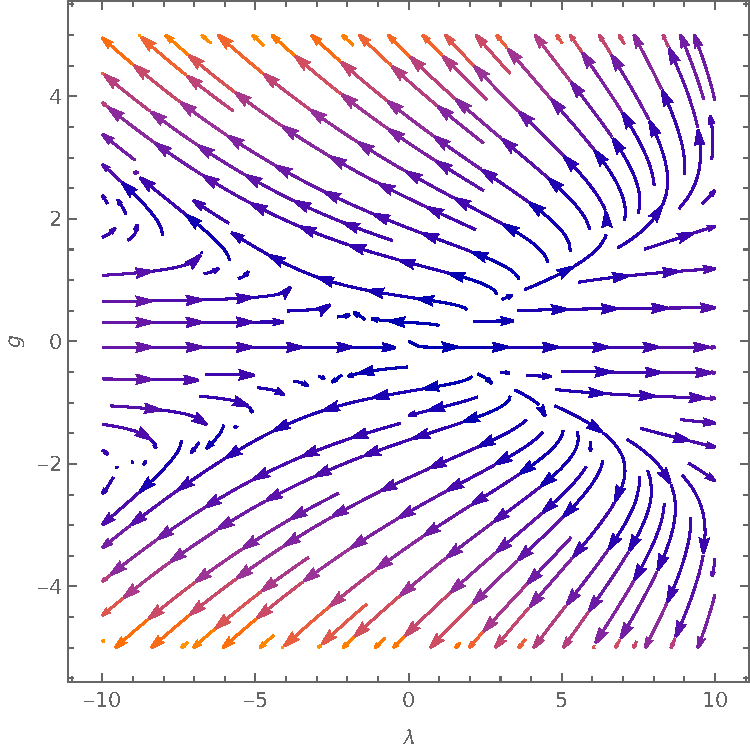
\includegraphics[width=.4\textwidth]{1}
		\caption{Coupling constant flow in the $\lam$-$g$ plane.}
		\label{f1}
	\end{figure}
}